\chapter{Big Example}
\label{chap:big_example}
This chapter demonstrates how Distrace can be used on bigger example and also serves as the user manual for creating custom monitoring applications. We will show how all steps from creating the application up to running the application and seeing the observed results.

This example is based on the H\textsubscript{2}O\footnote{More information about H\textsubscript{2}O can be found on \url{https://www.h2o.ai} and \url{https://github.com/h2oai}} open-source fast scalable machine learning platform. This platform supports various methods for building machine learning models, methods such as deep learning, gradient boosting or random forests. The core of the tool is written in Java and clients for different languages exist as well. Internally, H\textsubscript{2}O is using map-reduce computation paradigm\footnote{Map-reduce is a programming model in distributed systems. The basic idea is to split tasks into smaller parts and perform the map operations. The intermediate results are then combined together using the reduce calls until the complete result has been assembled from all the sub-tasks.} to perform various tasks across the cluster.

The goal of this example is to monitor subset of map-reduce tasks and see visualization of the computation process. This can help reasoning about performance of the platform and can discover unwanted delays in computations. This chapter first describes relevant parts of the H2O platform in more details. Then in the following sections we describe in steps how to extend the core instrumentation library for H2O purposes. Lastly, we show how this example can be started and how visual output can be interpreted. 
This full example is also available in the attached source code of the thesis.

\section{H\textsubscript{2}O In More Details}
H\textsubscript{2}O is in-memory machine learning platform. The computations are performed in cluster, where the cluster consists of several H2O nodes. All nodes in the cluster are equal and each of them can initialize the computation. Each computation is performed as a map-reduce. This section first describes the format of data used in H2O and how data are stored and then how the computations is performed in the cluster. 

\subsection{Data in H\textsubscript{2}O}
Data are stored in H\textsubscript{2}O in so called \texttt{Frames}. Frame is an in-memory distributed data table with columns and rows. The \texttt{Frame} is designed in a way that it can handle data which are not possible to fit into a memory of a single machine. Each column is represented by the \texttt{Vec} class. This class represents vector of data that is again distributed across nodes in the cluster. Further, each vector is split into multiple \texttt{Chunk}s, where chunk is part of the vector actually stored on the single node. 

It is possible for one node to contain multiple chunks from a single frame and therefore, the number of chunks in a vector does not represent the number of nodes on which the data are distributed. Also, data imported to H\textsubscript{2}O are distributed via chunks equally among all the nodes in the cluster, but algorithm may also decide to distribute the data on just several nodes in the cluster. It is also possible to create the frame manually and specify on which nodes the chunks should be stored. Therefore, the frame may be distributed on only a portion of the cluster. Also, usually when chunks are being created on some specific node, chunks of the same size for each column are created on that node. This means that each node storing the data usually have corresponding chunks for all the columns. This can be though of that each node storing some data has a subset of rows from the full table with all columns.

The Figure \ref{fig:h2o_frame} shows the structure of frame with three columns, where each column is split into two chunks. It also shows how chunks may be distributed in the cluster of size three. It can also be seen that corresponding chunks for each vector have the same size and are stored on the same nodes. 

	\begin{figure}
		\centering
		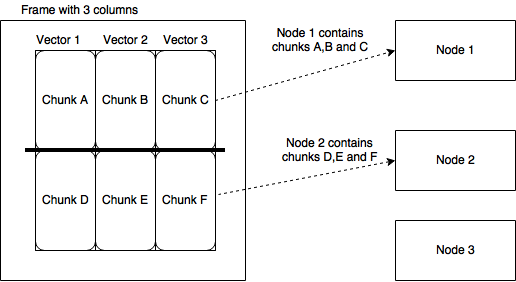
\includegraphics[scale=0.5]{h2o_frame.png}
		\caption{Structure of H\textsubscript{2}O frame and its distribution in the cluster.}
		\label{fig:h2o_frame}
	\end{figure}

\subsection{Computation in H\textsubscript{2}O}
For example, when the user tells H2O to create a deep learning model based in the data on the input, H2O sees this as a \textbf{Job}. Jobs are used to track long-lifetime user interactions and encapsulate the whole computation from the user point of view. The job can consist of several map-reduce tasks. In H2O, the class \texttt{MRTask} is used as the core implementation of the map-reduce tasks. The map-reduce task is always bound to some  H\textsubscript{2}O frames on which the computation needs to be performed. This class is used to encapsulate the task, partition it to a smaller tasks and run remote computations among the whole cluster. The \texttt{map} operations are called on the leaf tasks to compute the result based on the locally available data and \texttt{reduce} calls are used to reduce the result from two sub-tasks into a new task with combined result from the children.

In more detail, the class \texttt{MRTask} extends from \texttt{DTask}. This class is a general class used in H\textsubscript{2}O to represent task remote executed. Further, \texttt{DTask} extends from \texttt{H2OCountedCompleter}. The last class is a simple wrapper around the Fork/Join execution framework\footnote{For more information, please read Java documentation for Fork/Join framework available at \url{https://docs.oracle.com/javase/tutorial/essential/concurrency/forkjoin.html}.} allowing the platform to prioritize tasks. Fork/Join (F/J) framework is an implementation of Java \texttt{ExecutorService}, which helps with job parallelization on multiple processors. The Fork/Join thread framework execute tasks in separated threads and can move tasks between threads to ensure the highest possible performance. Each H\textsubscript{2}O \texttt{MRTask} is executed as \texttt{ForkJoinTask} inside this execution framework. A \texttt{ForkJoinTask} is a task wrapper which can run inside a single thread. It is a light-weight wrapper and big number of tasks may be served by a smaller number of actual threads.

The way how H\textsubscript{2}O perform computation from high-level point of view can be seen on the Figure \ref{fig:h2o_overview}. The task initiator receives the \texttt{MRTask} from the parent \texttt{Job} or from the user. It splits the task into two new sub-tasks and send these tasks to new nodes in the cluster. The intermediary nodes does the the splitting again and sends the task again to the another two selected nodes in the cluster. The leaf nodes does not split the task anymore.

	\begin{figure}
		\centering
		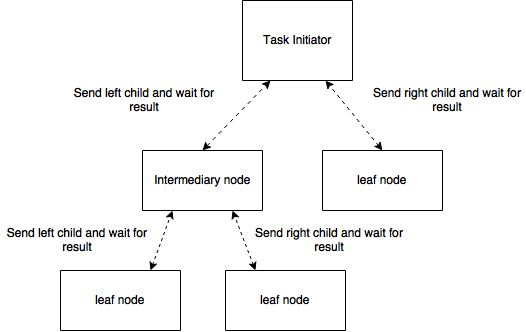
\includegraphics[scale=0.5]{h2o_overview.png}
		\caption{High-level overview of execution hierarchy.}
		\label{fig:h2o_overview}
	\end{figure}


It is important to say that the \texttt{MRTask} is always distributed to all nodes in the cluster. This figure shows how it is ensured that each node will be participating in the computation, however we still miss the computation step itself. Each node of the cluster who receives a task also submit this task for computation into the Fork/Join execution framework. This computation performs the mapping operation on all the chunks, which are available locally on the node executing this task, for the frame associated to the task. The \texttt{operation} follows the \texttt{map} operation, however we need to first ensure that the child tasks, from which we want to combine results together, are already finished. This is ensured by child tasks signaling the parent tasks when the work has been finished so parent tasks can know when they can start reducing the results.

The computation on the single node is shown in the following pseudo-code
\begin{lstlisting}[language=Java]
 MRTask task = ... // task received from the parent or from the user
 MRTask left = split(task, start1, end1)
 MRTask right = split(task, start2, end2)
 remoteCompute(left)
 remoteCompute(right)
 H2O.submitTask(task) // submit this task into F/J
..
// task is taken from F/J for execution
task.map(..)
task.waitForComplete() // wait for the child tasks to finish
task.reduce(left, right)

notifyComplete(task) // notify parent of completion
\end{lstlisting}
The split method accept also indices representing nodes in the cluster on which this sub-task and further sub-sub-tasks may be executed.

The last missing piece of information is what is done when the node has more chunks available for the frame associated with the task, since each \texttt{map} operation is executed only per single chunk. In case the node has multiple chunks available for the frame, the node always locally submits two new tasks into the F/J framework, each having half of the chunks. This is recursively repeated until we have tasks of size one chunk which are processed normally. These locally-split tasks signalize to their parents that they are done. This signalization goes up the tree until the original task is marked finished.

\subsection{Methods for Instrumentation}
For purpose of this example, a special \texttt{MRTask} called \texttt{SumMRTask} has been created. This task just perform distributed sum of the range of the numbers. In order to be able to visualize the computation process of this task, the following \texttt{MRtask} methods are important for the instrumentation
\begin{itemize}
	\item \texttt{dfork} - this method is called at the initiator node and starts the computation of the whole task.
	\item \texttt{getResult} - this method is also called at the initiator and blocks until the distributed computation finishes.
	\item \texttt{setupLocal0} - this method splits the task, creates sub-tasks for child nodes and finally submits the sub-tasks to the target child nodes.
	\item \texttt{map} - the map operation.
	\item \texttt{reduce2} - the reduce operation.
	\item \texttt{compute2} - this method handles the computation itself by calling the \texttt{map} implementation.
	\item \texttt{onComplete} - this method waits for the sub-tasks to finish and then calls \texttt{reduce2} on them.
\end{itemize}

We are also interested how long the remote computation lasted on child nodes. For this reason we need to instrument the following two methods on the \texttt{RPC} class:
\begin{itemize}
	\item \texttt{call} - this method is called when the remote computation has been submitted.
	\item \texttt{response} - this method is called when the remote computation has been finished and the child node is signaling that its work is done.
\end{itemize}

\section{Building the Core Server and Native Agent}
In order be able to extend the core instrumentation library, we need to build it first. This won't be necessary once the core instrumentation server is published to some online repository of JAR packages\footnote{For example, Maven Central Repository.} The native agent also needs to be built on the platfrom where H\textsubscript{2}O will be running.

To build the both parts, the developer needs to obtain the Distrace tool sources\footnote{Distrace is available at \url{https://github.com/jakubhava/Distrace}.} and call \texttt{./gradlew build}\footnote{On Windows, \texttt{./gradlew.bat build}} command, which builds the tool and produces artifacts for the core instrumentation server and the native agent as well. The build process requires several dependencies to be available on the machine such as Java virtual machine and Nanomsg and Nanomsgxx libraries.

In order to run this example without the need to set up these dependencies, the Docker container with this example is prepared. This container creates cluster of three H\textsubscript{2}O nodes with the agents attached and also starts the Zipkin user interface on the default port. To run the example in Docker, Docker needs to be available, the projects source directory needs to be available as well\footnote{The sources are not actually needed for running the examples in docker, but the script which is used to start the docker machines is available there as well.} and the following script should be called: \texttt{./docker/run-test.sh}\footnote{On Windows, \texttt{./docker/run-test.cmd}}. For more information how to start the examples in docker, please read the readme file in the source code directory.

\section{Extending the Core Instrumentation Server}

\section{Configuring and Running the Application}

\section{Interpreting the Results}